In this chapter, we describe the approach which we have adopted to create the dynamic benchmark of executable python software. The overall workflow of the approach is shown in the Figure \ref{fig:overall_approach}.

With the provided approach, our benchmark aims to achieve the properties of being large-scale, diverse, ready to run, ready to analyze, compositional and long term. We start with a large corpus of open source python projects, from which we select python projects for our benchmark (Section \ref{approach:selection of projects}). We then install and setup the selected python projects along with analysis tools and frameworks using bash scripts(Section \ref{approach:setup and install}). Furthermore, we create a single command line base interface to provide an easy access to the benchmark for execution of various tasks such as dynamic analysis, trace file generation, etc. (Section \ref{approach:command line interface}). Finally, we package and export our benchmark to be used by developers and researchers (Section \ref{approach: packing and exporting}). 

\begin{figure}[ht]
\centering
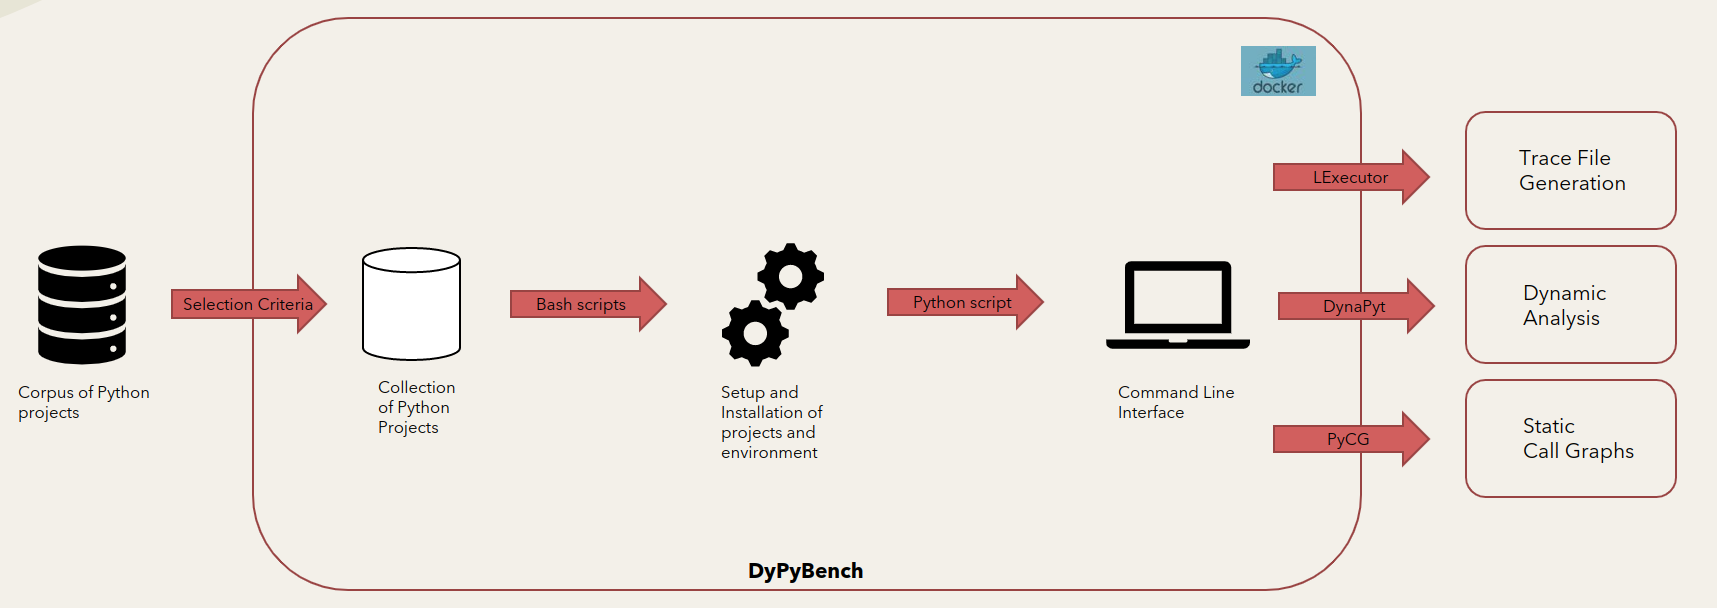
\includegraphics[width=1\linewidth]{figures/approach/Approach_final.png}
\caption[Approach]{\label{fig:overall_approach}Overall Approach of DyPyBench.}
\end{figure}

\section{Selection Criteria}
\label{approach:selection criteria}
The selection criteria enforces our benchmark to be large scale i.e., consisting of a large number of projects and diverse i.e., the projects must be from varied application domains. Github \cite{github} has a large number of open source projects written in the python programming languages which acts as a corpus for our benchmark. In order to select the projects which are well accepted in the community similar to the other accepted benchmarks such as ..., we add the criteria of a minimum threshold of stars on GitHub. We keep this threshold to be 1000 as too few stars would mean the project is not well accepted or is still pretty new, while 500 stars makes it popular but not so widely used. After filtering the projects based on GitHub stars, we select the projects from the corpus which belong to different application domains which are covered by the python projects. To name a few, the projects such as ... cover the domains ...respectively. Applying the selection criteria, we select 50 projects from the corpus of open source projects available on GitHub.

\section{Selected Python Projects}
\label{approach:selection of projects}
Since Python is a very popular and general purpose programming language, it has been used in many domains and we have a large set of open source python projects available on the internet. In this thesis we target projects from many of these varied domains which are well accepted in the community and at the same time open sourced. Another important factor is the availability of test suites in the project source code. 

\section{Setup and Install}
\label{approach:setup and install}
With a set of selected projects based on the required criteria, we then proceed to setup and install these projects with each one having its own virtual environment to install all the dependencies with their specific version from the requirements file. And then also using the source to install the project and its dependencies with pip package manager. Each of these projects are numbered and are placed inside their own folders. The projects source is cloned to a particular date. We also install some of the other python packages using pip in order to run the test suites successfully. We end the setup with installing the packages for testing and analysis tools present in the benchmark.

\section{Command Line Interface}
\label{approach:command line interface}
With the selected projects from section \ref{approach:selection of projects} installed and setup, we provide a command line interface for the user to run tests and dynamic analysis of a single project or a collection of projects. This command line interface is a single command with various available options. The various options available are to list all the installed projects with their urls, run the test suite of the project, perform instrumentation of the source code for dynamic analysis using dynapyt or lexecutor. execution of lexecurtor or dynapyt analysis. It also provides the option to update dynapyt and lexecutor. WE can also store the output to a particular file or spefic a timeout for the specific tasks where applicable. 

\section{Dynamic Analysis}
\label{approach:dynamic analysis}
While the command line interface provides us with varied options, one such option is the dynamic analysis. There are two available analysis, dynapyt and lexeecutor. We can use the command line to perform the specific analysis and generate the logs which we can use to train machine learning models for program analysis or use these logs on our own to understand the behaviour of the selected projects. These analysis can also help us in discovering some issues in the selected python projects. An example is dynapyt which explored a bug in pytorch. 

\section{ML Model}
\label{approach:ml model}

\section{Application}
\label{approach:application}